%%%%%%%%%%%%%%%%%%%%%%%%%%%%%%%%%%%%%%%%%%%%%%%%%%%%%%%%%%%%%%%%%%%%%%%%%%%%%%%%%%%
%% This project aims to create the UFC template for presentation.                %%
%% author: Maurício Moreira Neto - Doctoral student in Computer Science (MDCC)   %%
%% contacts:                                                                     %%
%%    e-mail: maumneto@ufc.br                                                    %%
%%    linktree: https://linktr.ee/maumneto                                       %%
%%%%%%%%%%%%%%%%%%%%%%%%%%%%%%%%%%%%%%%%%%%%%%%%%%%%%%%%%%%%%%%%%%%%%%%%%%%%%%%%%%%
\documentclass{libs/ufc_format}
% Inserting the preamble file with the packages
%%%%%%%%%%%%%%%%%%%%%%%%%%%%%%%%%%%%%%%%%%%%%%%%%%%%%%%%%%%%%%%%%%%%%
%% This file contains the packages that can be used in the beamer. %%
%%%%%%%%%%%%%%%%%%%%%%%%%%%%%%%%%%%%%%%%%%%%%%%%%%%%%%%%%%%%%%%%%%%%%
% Package to fonts family
\usepackage[T1]{fontenc}
% Package to accentuation
\usepackage[utf8]{inputenc}
% Package to Portuguese language
\usepackage[brazil]{babel}
% Package to Figures
\usepackage{graphicx}
% Package to the colors
\usepackage{color}
% Package to the colors
\usepackage{xcolor}
% Packages to math symbols and expressions
\usepackage{amsfonts, amssymb, amsmath}
% Package to multiple lines and columns in table
\usepackage{multirow, array} 
% Package to create pseudo-code
% For more detail of this package: http://linorg.usp.br/CTAN/macros/latex/contrib/algorithm2e/doc/algorithm2e.pdf
\usepackage{algorithm2e}
% Package to insert code
\usepackage{listings} 
\usepackage{keyval}
% Package to justify text
\usepackage[document]{ragged2e}
% Package to manage the bibliography
\usepackage[backend=biber, style=numeric, sorting=none]{biblatex}
% Package to facilities quotations
\usepackage{csquotes}
% Package to use multicols
\usepackage{multicol}


%% On my own
\newcommand{\aspas}[1]{``#1''}

% Inserting the references file
\bibliography{references.bib}
\usepackage{emoji}
\usepackage{longtable}
\usepackage{graphicx}
\usepackage{media9}
\usepackage{animate}

% Title
\title[Aprendizado Estatístico em Dados Longitudinais]{\huge\textbf{Aprendizado Estatístico em Dados Longitudinais}}
% Subtitle
\subtitle{}
% Author of the presentation
\author{Cícero Hitzschky}
% Institute's Name
\institute[UFC]{
    % email for contact
    \normalsize{\email{cicero.hitzschky@alu.ufc.br}}
    \newline
    % Department Name
    \department{Departamento de Estatística e Matemática Aplicada}
    \newline
    % university name
    \ufc
}
% date of the presentation
\date{\today}


%%%%%%%%%%%%%%%%%%%%%%%%%%%%%%%%%%%%%%%%%%%%%%%%%%%%%%%%%%%%%%%%%%%%%%%%%%%%%%%%%%
%% Start Document of the Presentation                                           %%               
%%%%%%%%%%%%%%%%%%%%%%%%%%%%%%%%%%%%%%%%%%%%%%%%%%%%%%%%%%%%%%%%%%%%%%%%%%%%%%%%%%
\begin{document}
% insert the code style
%%%%%%%%%%%%%%%%%%%%%%%%%%%%%%%%%%%%%%%%%%%%%%%%%%%%%%%%%%%%%%%%%%%%%%%%%%%%%%%%%%%
%% This file contains the style of the codes show in slides.                     %%
%% The package used is listings, but it possible to used others.                 %%
%%%%%%%%%%%%%%%%%%%%%%%%%%%%%%%%%%%%%%%%%%%%%%%%%%%%%%%%%%%%%%%%%%%%%%%%%%%%%%%%%%%

% color used in the code style
\definecolor{codegreen}{rgb}{0,0.6,0}
\definecolor{codegray}{rgb}{0.5,0.5,0.5}
\definecolor{codepurple}{rgb}{0.58,0,0.82}
\definecolor{codebackground}{rgb}{0.95,0.95,0.92}

% style of the code!
\lstdefinestyle{codestyle}{
    backgroundcolor=\color{codebackground},   
    commentstyle=\color{codegreen},
    keywordstyle=\color{magenta},
    numberstyle=\tiny\color{codegray},
    stringstyle=\color{codepurple},
    basicstyle=\ttfamily\footnotesize,
    frame=single,
    breakatwhitespace=false,         
    breaklines=true,                 
    captionpos=b,                    
    keepspaces=true,                 
    numbers=left,                    
    numbersep=5pt,                  
    showspaces=false,                
    showstringspaces=false,
    showtabs=false,                  
    tabsize=2,
    title=\lstname 
}

\lstset{style=codestyle}


%% ---------------------------------------------------------------------------
% First frame (with tile, subtitle, ...)
\begin{frame}{}
    \maketitle
\end{frame}

%% ---------------------------------------------------------------------------
% Second frame
\begin{frame}{Sumário}
    \begin{multicols}{2}
        \tableofcontents
    \end{multicols}
\end{frame}

%% ---------------------------------------------------------------------------
% This presentation is separated by sections and subsections


\section{Inteligencia Artificial}
\subsection{O que é Inteligência Artificial?}
\begin{frame}{O que é inteligência Artificial (IA)?}
    \begin{block}{}
        \begin{itemize}
            \item Não existe uma definição exata.
            \item Depende do contexto em que está empregada.
        \end{itemize}
    \end{block}
\end{frame}
% John Haugeland
\begin{frame}{O que é IA?}
    \begin{minipage}{0.5\linewidth}
        \begin{figure}
            \centering
            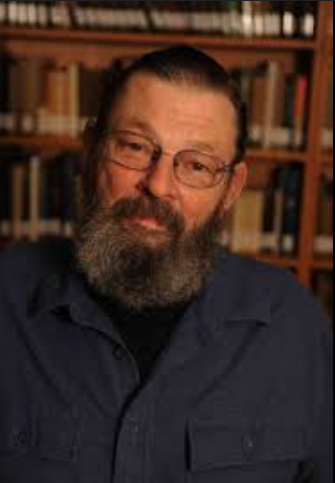
\includegraphics[width=0.6\linewidth]{imagens//secao1/haugeland1985.png}
            \caption{Prof. John Haugeland}
        \end{figure}
    \end{minipage}
    \begin{minipage}{0.5\linewidth}
        \begin{itemize}
        \justifying
            \item \textit{Artificial Intelligence: The Very Idea (1985).}
            \item \aspas{O novo e interessante esforço para fazer os
        computadores pensarem (...) máquinas com mentes, no
        sentido total e literal.}
        \end{itemize}
    \end{minipage}
\end{frame}

% Richard Bellman
\begin{frame}{O que é IA?}
    \begin{minipage}{0.5\linewidth}
        \begin{itemize}
        \justifying
            \item \textit{Artificial Intelligence (1972).}
            \item 
            \aspas{[Automatização de] atividades que associamos ao pensamento humano, atividades como a tomada de decisões, a resolução de problemas, o aprendizado...}
        \end{itemize}
    \end{minipage}
    \begin{minipage}{0.5\linewidth}
        \begin{figure}
            \centering
            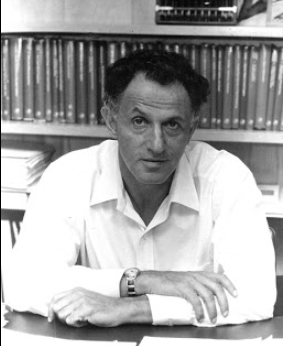
\includegraphics[width=0.6\linewidth]{imagens//secao1/bellman1978.png}
            \caption{Richard Bellman}
            \label{fig:enter-label}
        \end{figure}
    \end{minipage}
\end{frame}

% Raymond Kurzweil
\begin{frame}{O que é IA?}
    \begin{minipage}{0.5\linewidth}
        \begin{figure}
            \centering
            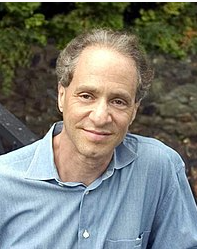
\includegraphics[width=0.5\linewidth]{imagens//secao1/kurzweil.png}
            \caption{Raymond Kurzweil}
        \end{figure}
    \end{minipage}
    \begin{minipage}{0.5\linewidth}
        \begin{itemize}
        \justifying
            \item \textit{The Age of Intelligent Machines (1990).}
            \item 
            \aspas{A arte de criar máquinas que executam funções que exigem inteligência quando executadas por pessoas.”}
        \end{itemize}
    \end{minipage}
\end{frame}

\begin{frame}{O que é IA? }
    \begin{itemize}
        \item 
        \aspas{
        O estudo das faculdades mentais pelo uso de modelos computacionais.
        }
        (Charniak e McDermott, 1985) 
        
        \item 
        \aspas{
        O estudo das computações que tornam possívelperceber, raciocinar e agir.
        }
        (Winston, 1992)
        
        \item 
        \aspas{
        O estudo de como os computadores podem fazer tarefas que hoje são melhor desempenhadas pelas pessoas.
        }
        (Rich and Knight, 1991)
        
        \item 
        \aspas{
        “Inteligência Computacional é o estudo do projeto de agentes inteligentes.
        }
        (Poole et al., 1998) 

        \item 
        \aspas{
        AI... está relacionada a um desempenho inteligente de artefatos.
        }
        (Nilsson, 1998)
    \end{itemize}
\end{frame}
\section{Diferenças entre Abordagem Estatística Tradicional e Aprendizado Estatístico}

\begin{frame}{}
	\begin{figure}[h]
		
\includegraphics[scale=0.4]{imagens//secao2/artigo1.png}
	\end{figure}
\end{frame}


\begin{frame}{Possíveis complicações com abordagem Estatística Tradicional em Dados Longitudinais}
    \begin{block}{}
        \begin{itemize}
            \item Geralmente exigem técnicas mais avançadas;
            \item Herança de suposições, e.g, homoscedasticidade, normalidade, independência de observações, falta correlação entre variáveis preditoras...
        \end{itemize}
    \end{block}
\end{frame}

\begin{frame}{Suposições de alguns modelos estatísticos}
	\begin{block}{Modelos de Efeitos Fixos}
		\begin{itemize}
			\item Independência Condicional: Dados os efeitos fixos, os erros são independentes;
			\item Ausência de Correlação Serial; 
			\item O erro aleatório é não correlacionado ao longo do tempo;
			\item Homoscedasticidade dos resíduos.
		\end{itemize}
	\end{block}
\end{frame}

\begin{frame}{Suposições de alguns modelos estatísticos}
	\begin{block}{Modelos de Efeitos Aleatórios}
		\begin{itemize}
			\item Normalidade dos componentes aleatórios bem como dos resíduos;
			\item Homoscedasticidade; 
			\item Ausência de correlação serial.
		\end{itemize}
	\end{block}
\end{frame}

\begin{frame}{Suposições de alguns modelos de Aprendizado Estatísticos}
	\begin{block}{Naive Bayes}
		Independência dos preditores.
	\end{block}
	\begin{block}{Floresta Aleatória}
		Nenhum dado ausente.
	\end{block}
	\begin{block}{Redes Neurais}
		Nenhum dado ausente.
	\end{block}
	\begin{block}{Gradient Boosting}
		Nenhuma suposição inicial.
	\end{block}
\end{frame}

\begin{frame}{Comparação: Estatística Tradicional vs. Aprendizado Estatístico}
	\resizebox{\linewidth}{!}{
		\begin{tabular}{p{4cm} p{5cm} p{5cm}}
		\textbf{Atributo} & \textbf{Estatística Tradicional} & \textbf{Aprendizado de Máquina} \\
		\hline
		Adequado para & 
		Teste de hipóteses dedutivas &
		Geração de hipóteses abdutivas \\
		
		\hline 
		Forma das relações entre variáveis &
		Ajusta os dados em formas predefinidas especificadas no modelo estatístico &
		Aprende a verdadeira forma da relação entre variáveis \\
		
		\hline
		Objetivo principal &
		Testar se existem relacionamentos pré-especificados nos dados &
		Identificar padrões nos dados sem preconceitos \\
		
		\hline 
		Padrão geral de resultados &
		Baixa previsibilidade, alta explicabilidade &
		Alta previsibilidade, baixa explicabilidade \\
	\end{tabular}
	}
\end{frame}


\begin{frame}{Comparação: Estatística Tradicional vs. Aprendizado Estatístico}
	\resizebox{\linewidth}{!}{
		\begin{tabular}{p{5cm} p{4cm} p{4cm}}
			\textbf{Atributo} & \textbf{Estatística Tradicional} & \textbf{Aprendizado de 	Máquina} \\		
			\hline			
			Como confiar na análise &
			Testes de robustez &
			Modelo de teste em dados não vistos. 
			Teste a generalização por meio de análise secundária \\
			\hline
			Experiência necessária &
			Experiência em modelos estatísticos &
			Experiência em análise de diversos conjuntos de dados \\
			\hline 
			Habilidades de pesquisador &
			Treinamento em estatística &
			Treinamento em ciência de dados e programação \\

		\end{tabular}
	}
\end{frame}


\begin{frame}{Comparação: Estatística Tradicional vs. Aprendizado Estatístico}
	\resizebox{\linewidth}{!}{
	\begin{tabular}{p{3.5cm} p{4.5cm} p{4.5cm}}
		\textbf{Atributo} & \textbf{Estatística Tradicional} & \textbf{Aprendizado de Máquina} \\
		\hline 
		Poder computacional Exigido &
		Laptops modernos geralmente são suficientes &
		Requer ambiente de computação de ponta \\
		\hline
		Reutilização de modelos & 
		Precisa construir modelos diferentes para cada objetivo &
		Um algoritmo pode ser reutilizado para diferentes objetivos \\
		\hline
		Número de preditores &
		Limitado pela correlação entre variáveis &
		Limitado pelo poder computacional \\
	\end{tabular}}
\end{frame}














\section{Aplicação}

\begin{frame}{Contextualização}
	\begin{block}{Osteoporose}
		é uma doença em que a degradação estrutural e a diminuição da densidade mineral dos ossos (DMO) aumentam o risco de fraturas ósseas.
	\end{block}
	\begin{block}{Motivações para o estudo}
		\begin{itemize}
			\item  A prevalência da osteoporose aumentou drasticamente nos últimos anos;
			\item  Representa um problema de saúde pública com alto índice de morbidade (muito comum).
		\end{itemize}
	\end{block}
\end{frame}

\begin{frame}{Contextualização}
	\begin{block}{}
		\begin{itemize}
			\item Em 2010, na União Europeia, aproximadamente 5,5 milhões de homens e 22 milhões de mulheres foram afetados pela osteoporose;
			\item 80\% das mulheres afetadas não estavam cientes dos seus fatores de risco até o diagnóstico.
		\end{itemize}
	\end{block}
\end{frame}

\begin{frame}{Objetivos}
	\begin{block}{}
			\begin{enumerate}
			\item Comparar a precisão preditiva dos métodos aprendizado de máquina com a regressão linear múltipla tradicional;
			\item Classificar a importância de vários fatores de risco, incluindo dados demográficos, estilo de vida e bioquímica, na previsão das mudanças futuras no $\delta$-T score.
		\end{enumerate}
	\end{block}
\end{frame}

\begin{frame}{Metodologia}
\end{frame}
\begin{frame}{Fonte dos Dados}
	\begin{itemize}
		\item Coorte MJ de Taiwan  
		\begin{itemize}
			\item Coorte prospectiva em andamento  
			\item Exames conduzidos pelos Centros de Triagem de Saúde MJ  
		\end{itemize}
	\end{itemize}
\end{frame}

\begin{frame}{Informações Coletadas}
	\begin{itemize}
		\item Mais de 100 indicadores biológicos essenciais  
		\item Questionário abrangendo:  
		\begin{itemize}
			\item Histórico médico pessoal e familiar  
			\item Estado de saúde atual  
			\item Estilo de vida e exercício físico  
			\item Hábitos de sono e alimentares  
		\end{itemize}
	\end{itemize}
\end{frame}

\begin{frame}{Considerações Éticas}
	\begin{itemize}
		\item Consentimento informado dos participantes  
		\item Aprovação pelo Comitê de Ética
	\end{itemize}
\end{frame}

\begin{frame}{Modelos Utilizados}
	\begin{itemize}
		\item Floresta Aleatória (RF)
		\begin{itemize}
			\item É baseado em árvores de decisão que combina as técnicas de bagging e boosting.
			\item Minimiza a função de perda e resolve o sobreajuste das árvores de decisão tradicionais.
		\end{itemize}
	\end{itemize}
\end{frame}

\begin{frame}{Modelos Utilizados}
	\begin{itemize}
		\item Gradient Boosting Estocástico (SGB)
		\begin{itemize}
			\item Classifica objetos com base em características e variáveis específicas.
			\item Utiliza o teorema de Bayes para calcular a probabilidade das hipóteses sobre grupos presumidos.
		\end{itemize}
	\end{itemize}
\end{frame}

\begin{frame}{Modelos Utilizados}
	\begin{itemize}
		\item Naive Bayes (NB)
		\begin{itemize}
			\item Classifica objetos com base em características e variáveis específicas.
			\item Utiliza o teorema de Bayes para calcular a probabilidade das hipóteses sobre grupos presumidos.
		\end{itemize}
	\end{itemize}
\end{frame}

\begin{frame}{Modelos Utilizados}
	\begin{itemize}
		\item Extreme Gradient Boosting (XGBoost)
		\begin{itemize}
			\item Tecnologia de gradient boosting baseada na extensão otimizada do SGB.
			\item Treina vários modelos “fracos” e faz ensemble com o Gradiente Boosting.
		\end{itemize}
	\end{itemize}
\end{frame}










%\section{Seção I}
%\begin{frame}{Explicações}
%    % itemize
%    Este é um template que pode ser utilizado para \nocite{Template_Beamer_UFC}:
%    \begin{itemize}
%        \item Apresentação de Trabalhos Acadêmicos
%        \item Apresentação de Disciplinas
%        \item Apresentações de Teses e Dissertações
%    \end{itemize}
%
%    \vspace{0.4cm} % vertical space
%    
%    % enumeration
%    Para utilizar este template corretamente é importante que:
%    \begin{enumerate}
%        \item Tenha conhecimento mínimo sobre LaTeX
%        \item Ler os comentários no template (explicações)
%        \item Ler o README.md (documentação)
%    \end{enumerate}
%
%    \vspace{0.2cm}
%
%    \example{Este é um texto de exemplo!} \emph{Texto de Ênfase!}
%\end{frame}
%
%%% ---------------------------------------------------------------------------
%\subsection{Subseção I}
%\begin{frame}{Criando Blocos}
%    % Blocks styles
%    \begin{block}{Bloco Padrão}
%        Texto do corpo do bloco.
%    \end{block}
%
%    \begin{alertblock}{Bloco de Alerta}
%        Texto do corpo do bloco.
%    \end{alertblock}
%
%    \begin{exampleblock}{Bloco de Exemplo}
%        Texto do corpo do bloco.
%    \end{exampleblock}   
%\end{frame}
%
%%% ---------------------------------------------------------------------------
%\subsection{Subseção II}
%\begin{frame}{Criando Caixas}
%    \successbox{testando o success box}
%
%    \pause
%
%    \alertbox{testando o alert box}
%
%    \pause
%
%    \simplebox{testando o simple box}
%\end{frame}
%
%%% ---------------------------------------------------------------------------
%\subsection{Subseção III}
%\begin{frame}{Criando Algoritmos (Pseudocódigo)}
%    \begin{algorithm}[H]
%        \SetAlgoLined
%        \LinesNumbered
%        \SetKwInOut{Input}{input}
%        \SetKwInOut{Output}{output}
%        \Input{x: float, y: float}
%        \Output{r: float}
%        \While{True}{
%          r = x + y\;
%          \eIf{r >= 30}{
%           ``O valor de $r$ é maior ou iqual a 10.''\;
%           break\;
%           }{
%           ``O valor de $r$ = '', r\;
%          }
%         } 
%         \caption{Algorithm Example}
%    \end{algorithm}
%\end{frame}
%
%%% ---------------------------------------------------------------------------
%
%\begin{frame}{Inserindo Algoritmos}
%    \lstset{language=Python}
%    \lstinputlisting[language=Python]{code/main.py}
%\end{frame}
%
%%% ---------------------------------------------------------------------------
%\begin{frame}{Inserindo Algoritmos}
%    \lstinputlisting[language=C]{code/source.c}
%\end{frame}
%
%%% ---------------------------------------------------------------------------
%\begin{frame}{Inserindo Algoritmos}
%    \lstinputlisting[language=Java]{code/helloworld.java}
%\end{frame}
%
%%% ---------------------------------------------------------------------------
%\begin{frame}{Inserindo Algoritmos}
%    \lstinputlisting[language=HTML]{code/index.html}
%\end{frame}
%
%%% ---------------------------------------------------------------------------
%% This frame show an example to insert multicolumns
%\section{Multicolunas}
%\begin{frame}{Seção II - Multicolunas}
%    \begin{columns}{}
%        \begin{column}{0.5\textwidth}
%            \justify
%            É possível colocar mais de uma coluna utilizando os comandos de $\backslash$begin\{column\}\{\} e $\backslash$end\{column\}
%        \end{column}
%        \begin{column}{0.5\textwidth}
%            \justify
%            Porém, o espaçamento deve ser proporcional entre as colunas para que estas colunas não entrem em coflito. O espaçamento é dado pelo segundo argumento do $\backslash$begin.
%        \end{column}
%    \end{columns}    
%\end{frame}
%
%%% ---------------------------------------------------------------------------
%% This frame show an example to insert figures
%\section{Imagens}
%\begin{frame}{Seção III - Figures}
%    \begin{figure}
%        \centering
%        \caption{Emblema da UFC.}
%        
\includegraphics[scale=0.3]{libs/emblemufc.pdf}
%        \source{Obtido pelo site oficial da UFC \cite{siteufc} \cite{einstein}}
%        \label{fig:ufc_emblem}
%    \end{figure}
%\end{frame}
%
%% ---------------------------------------------------------------------------
% Reference frames
\begin{frame}{Referências}
    \begin{itemize}
    	\justifying
    	\item CHANG, Ching-Yao; PENG, Chung-Hsin; CHEN, Fang-Yu; HUANG, Li-Ying; KUO, Chun-Heng; CHU, Ta-Wei; LIANG, Yao-Jen. \textbf{The risk factors determined by four machine learning methods for the change of difference of bone mineral density in post-menopausal women after three years follow-up}. \textit{Scientific Reports}, [S. l.], v. 14, n. 1, p. 23234, dez. 2024. DOI: \url{https://doi.org/10.1038/s41598-024-73799-6}. Disponível em: <\url{https://www.nature.com/articles/s41598-024-73799-6}>. Acesso em: 28/02/2025.
    \end{itemize}
\end{frame}

\begin{frame}{Referências}
    \begin{itemize}
	   	\justifying
		\item SHEETAL, Abhishek; JIANG, Zhou; MILLA, Lee Di. \textbf{Using machine learning to analyze longitudinal data: A tutorial guide and best-practice recommendations for social science researchers}. \textit{Applied Psychology}, [S. l.], 25 set. 2022. DOI: \url{https://doi.org/10.1111/apps.12435}. Disponível em: <\url{https://doi.org/10.1111/apps.12435}>. Acesso em: 28/02/2025.
\end{itemize}
\end{frame}

\begin{frame}{Referências}
	\begin{itemize}
		\justifying
        \item GÉRON, Aurélien. \textbf{Hands-On Machine Learning with Scikit-Learn, Keras, and TensorFlow: Concepts, Tools, and Techniques to Build Intelligent Systems}. 2. ed. [S. l.]: O'Reilly Media, 2019.
        \item CARVALHO, Andz'
	\end{itemize}
\end{frame}



%% ---------------------------------------------------------------------------
% Final frame
\begin{frame}{}
    \centering
    \huge{\textbf{\example{Obrigado pela atenção!!!}}}
    
    \vspace{1cm}
    
    \Large{\textbf{Contato:}}
    \newline
    \vspace*{0.5cm}
    \large{\email{cicero.hitzschky@alu.ufc.br}}
\end{frame}

\end{document}